%%%%%%%%%%%%%%%%%%%%%%%%%%%%%%%%%%%%%%%%%
% LaTeX Template
%
% This template originates from:
% http://www.LaTeXTemplates.com
%
% License:
% CC BY-NC-SA 3.0 (http://creativecommons.org/licenses/by-nc-sa/3.0/)
% 
%%%%%%%%%%%%%%%%%%%%%%%%%%%%%%%%%%%%%%%%%

%----------------------------------------------------------------------------------------
%	PACKAGES AND OTHER DOCUMENT CONFIGURATIONS
%----------------------------------------------------------------------------------------

\documentclass{article}

%%%%%%%%%%%%%%%%%%%%%%%%%%%%%%%%%%%%%%%%%
% Lachaise Assignment
% Structure Specification File
% Version 1.0 (26/6/2018)
%
% This template originates from:
% http://www.LaTeXTemplates.com
%
% Authors:
% Marion Lachaise & François Févotte
% Vel (vel@LaTeXTemplates.com)
%
% License:
% CC BY-NC-SA 3.0 (http://creativecommons.org/licenses/by-nc-sa/3.0/)
% 
%%%%%%%%%%%%%%%%%%%%%%%%%%%%%%%%%%%%%%%%%

%----------------------------------------------------------------------------------------
%	PACKAGES AND OTHER DOCUMENT CONFIGURATIONS
%----------------------------------------------------------------------------------------

\usepackage{amsmath,amsfonts,stmaryrd,amssymb} % Math packages

\usepackage{enumerate} % Custom item numbers for enumerations

\usepackage[ruled]{algorithm2e} % Algorithms

\usepackage[framemethod=tikz]{mdframed} % Allows defining custom boxed/framed environments

\usepackage{listings} % File listings, with syntax highlighting
\lstset{
	basicstyle=\ttfamily, % Typeset listings in monospace font
}

%----------------------------------------------------------------------------------------
%	DOCUMENT MARGINS
%----------------------------------------------------------------------------------------

\usepackage{geometry} % Required for adjusting page dimensions and margins

\geometry{
	paper=a4paper, % Paper size, change to letterpaper for US letter size
	top=2.5cm, % Top margin
	bottom=3cm, % Bottom margin
	left=2.5cm, % Left margin
	right=2.5cm, % Right margin
	headheight=14pt, % Header height
	footskip=1.5cm, % Space from the bottom margin to the baseline of the footer
	headsep=1.2cm, % Space from the top margin to the baseline of the header
	%showframe, % Uncomment to show how the type block is set on the page
}

%----------------------------------------------------------------------------------------
%	FONTS
%----------------------------------------------------------------------------------------

\usepackage[utf8]{inputenc} % Required for inputting international characters
\usepackage[T1]{fontenc} % Output font encoding for international characters

\usepackage{XCharter} % Use the XCharter fonts

%----------------------------------------------------------------------------------------
%	COMMAND LINE ENVIRONMENT
%----------------------------------------------------------------------------------------

% Usage:
% \begin{commandline}
%	\begin{verbatim}
%		$ ls
%		
%		Applications	Desktop	...
%	\end{verbatim}
% \end{commandline}

\mdfdefinestyle{commandline}{
	leftmargin=10pt,
	rightmargin=10pt,
	innerleftmargin=15pt,
	middlelinecolor=black!50!white,
	middlelinewidth=2pt,
	frametitlerule=false,
	backgroundcolor=black!5!white,
	frametitle={Command Line},
	frametitlefont={\normalfont\sffamily\color{white}\hspace{-1em}},
	frametitlebackgroundcolor=black!50!white,
	nobreak,
}

% Define a custom environment for command-line snapshots
\newenvironment{commandline}{
	\medskip
	\begin{mdframed}[style=commandline]
}{
	\end{mdframed}
	\medskip
}

%----------------------------------------------------------------------------------------
%	FILE CONTENTS ENVIRONMENT
%----------------------------------------------------------------------------------------

% Usage:
% \begin{file}[optional filename, defaults to "File"]
%	File contents, for example, with a listings environment
% \end{file}

\mdfdefinestyle{file}{
	innertopmargin=1.6\baselineskip,
	innerbottommargin=0.8\baselineskip,
	topline=false, bottomline=false,
	leftline=false, rightline=false,
	leftmargin=2cm,
	rightmargin=2cm,
	singleextra={%
		\draw[fill=black!10!white](P)++(0,-1.2em)rectangle(P-|O);
		\node[anchor=north west]
		at(P-|O){\ttfamily\mdfilename};
		%
		\def\l{3em}
		\draw(O-|P)++(-\l,0)--++(\l,\l)--(P)--(P-|O)--(O)--cycle;
		\draw(O-|P)++(-\l,0)--++(0,\l)--++(\l,0);
	},
	nobreak,
}

% Define a custom environment for file contents
\newenvironment{file}[1][File]{ % Set the default filename to "File"
	\medskip
	\newcommand{\mdfilename}{#1}
	\begin{mdframed}[style=file]
}{
	\end{mdframed}
	\medskip
}

%----------------------------------------------------------------------------------------
%	NUMBERED QUESTIONS ENVIRONMENT
%----------------------------------------------------------------------------------------

% Usage:
% \begin{question}[optional title]
%	Question contents
% \end{question}

\mdfdefinestyle{question}{
	innertopmargin=1.2\baselineskip,
	innerbottommargin=0.8\baselineskip,
	roundcorner=5pt,
	nobreak,
	singleextra={%
		\draw(P-|O)node[xshift=1em,anchor=west,fill=white,draw,rounded corners=5pt]{%
		Question \theQuestion\questionTitle};
	},
}

\newcounter{Question} % Stores the current question number that gets iterated with each new question

% Define a custom environment for numbered questions
\newenvironment{question}[1][\unskip]{
	\bigskip
	\stepcounter{Question}
	\newcommand{\questionTitle}{~#1}
	\begin{mdframed}[style=question]
}{
	\end{mdframed}
	\medskip
}

%----------------------------------------------------------------------------------------
%	WARNING TEXT ENVIRONMENT
%----------------------------------------------------------------------------------------

% Usage:
% \begin{warn}[optional title, defaults to "Warning:"]
%	Contents
% \end{warn}

\mdfdefinestyle{warning}{
	topline=false, bottomline=false,
	leftline=false, rightline=false,
	nobreak,
	singleextra={%
		\draw(P-|O)++(-0.5em,0)node(tmp1){};
		\draw(P-|O)++(0.5em,0)node(tmp2){};
		\fill[black,rotate around={45:(P-|O)}](tmp1)rectangle(tmp2);
		\node at(P-|O){\color{white}\scriptsize\bf !};
		\draw[very thick](P-|O)++(0,-1em)--(O);%--(O-|P);
	}
}

% Define a custom environment for warning text
\newenvironment{warn}[1][Warning:]{ % Set the default warning to "Warning:"
	\medskip
	\begin{mdframed}[style=warning]
		\noindent{\textbf{#1}}
}{
	\end{mdframed}
}

%----------------------------------------------------------------------------------------
%	INFORMATION ENVIRONMENT
%----------------------------------------------------------------------------------------

% Usage:
% \begin{info}[optional title, defaults to "Info:"]
% 	contents
% 	\end{info}

\mdfdefinestyle{info}{%
	topline=false, bottomline=false,
	leftline=false, rightline=false,
	nobreak,
	singleextra={%
		\fill[black](P-|O)circle[radius=0.4em];
		\node at(P-|O){\color{white}\scriptsize\bf i};
		\draw[very thick](P-|O)++(0,-0.8em)--(O);%--(O-|P);
	}
}

% Define a custom environment for information
\newenvironment{info}[1][Info:]{ % Set the default title to "Info:"
	\medskip
	\begin{mdframed}[style=info]
		\noindent{\textbf{#1}}
}{
	\end{mdframed}
}
 % Include the file specifying the document structure and custom commands

\usepackage{graphicx}
%Path in Windows format:
\graphicspath{ {.Images/} }

%----------------------------------------------------------------------------------------
%	ASSIGNMENT INFORMATION
%----------------------------------------------------------------------------------------

\title{Gambler's Ruin - Theory} % Title of the assignment

\author{Tansel Arif\\ \texttt{tanselarif@live.co.uk}} % Author name and email address

\date{\today} % University, school and/or department name(s) and a date

%----------------------------------------------------------------------------------------

\begin{document}

\maketitle % Print the title

%----------------------------------------------------------------------------------------
%	INTRODUCTION
%----------------------------------------------------------------------------------------

\section*{Introduction} % Unnumbered section

The Gambler's Ruin problem frames a gambler who begins gambling with an initial fortune - in dollars say. At each successive gamble, the gambler either loses \$1 or gains \$1. The problem is to find the probability that the gambler goes bankrupt - loses the entirety of the fortune. This problem is a kind of random walk. Figures \ref{fig:sim1} and \ref{fig:sim2} below show simulation trajectories for this setup.

\begin{figure}[r]
    \centering
    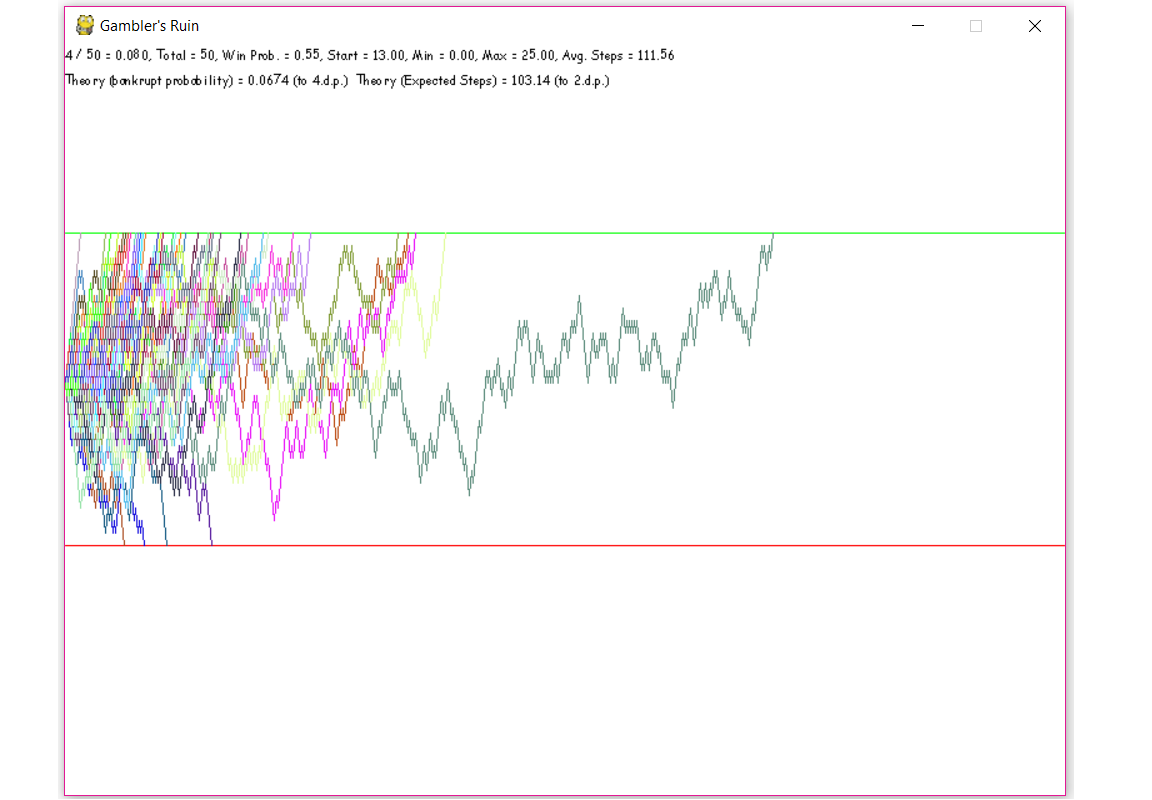
\includegraphics[width=\textwidth]{Simulation1}
    \caption{This is a plot of 10 simulations with $k = 12.5$, $p = 0.55$, $N = 25$. The theory results in a probability of 0.0753 of bankruptcy. The horizontal green line represents \$N and the hosrizontal red line represents \$0.}
    \label{fig:sim1}
\end{figure}

\begin{figure}[r]
    \centering
    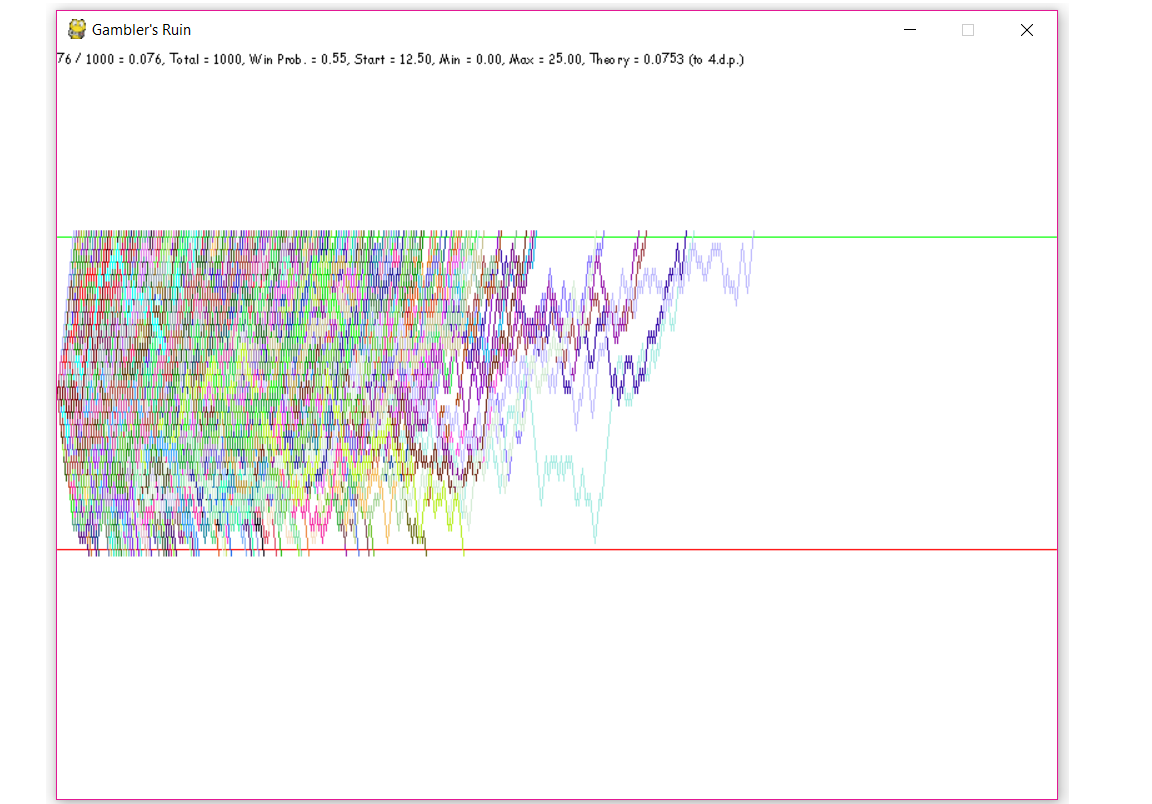
\includegraphics[width=\textwidth]{Simulation2}
    \caption{This is a plot of 1000 simulations with $k = 12.5$, $p = 0.55$, $N = 25$. The theory results in a probability of 0.0753 of bankruptcy. The horizontal green line represents \$N and the hosrizontal red line represents \$0.}
    \label{fig:sim2}
\end{figure}

\section{The Problem} % Numbered section

A Gambler begins with \$k and repeatedly plays a game after which they may win \$1 with probability $p$ or lose \$1 with probability $q=1-p$. The Gambler will stop playing if their fortune reaches \$0 or \$N. What is the probability that they go bankrupt?

\section{The Solution} % Numbered section

Let $u_k$ be the probability that the Gambler bankrupts if the initial fortune is \$k. Then we can condition this probability on the first gamble as follows (utilising the law of total probability with the partitioning of lose/win):

$$u_k = P(wins) \times u_{k+1} + P(loses) \times u_{k-1}$$

This is a second order homogeneous difference equation. We look for solutions of the form $u_n = A \times \lambda^n$.

$$p \times u_{n+1} - u_n + q u_{n-1} = 0$$
$$\implies p \times A \times \lambda^{n+1} - A \times \lambda^n + q \times A \times \lambda^{n-1} = 0$$
$$\implies \lambda^{2} - \frac{1}{p} \lambda + \frac{q}{p} = 0$$

where $p, q \neq 0$. This has solution:

$$\lambda_{1,2} = \left\{\frac{1-p}{p},1\right\}$$

provided that $p \neq \frac{1}{2}$, this gives 2 different solutions. We have:

$$u_n = A \left( \frac{1-p}{p} \right)^n + B (1)^n$$
$$ = A \left( \frac{1-p}{p} \right)^n + B$$

We have that the Gambler stops gambling if either their fortune reaches \$0 or \$N. So we have the following boundary conditions:

$$u_0 = 1, u_N = 0$$

Using these boundary conditions, we can solve for $A$ and $B$:

$$u_0 = A \left( \frac{1-p}{p} \right)^0 + B = 1$$
$$\implies A+B = 1$$
$$\implies B = 1 - A$$

and

$$u_N = A \left( \frac{1-p}{p} \right)^N + B = 0$$
$$\implies B = -A \left( \frac{1-p}{p} \right)^N$$
$$\implies 1 - A = -A \left( \frac{1-p}{p} \right)^N$$
$$\implies A = \frac{1}{1 - \left( \frac{1-p}{p} \right)^N}$$
$$\implies B = 1-A = \frac{-\left( \frac{1-p}{p} \right)^N}{1 - \left( \frac{1-p}{p} \right)^N}$$

Giving the final solution:

\begin{equation}
    u_n = \frac{\left( \frac{1-p}{p} \right)^n-\left( \frac{1-p}{p} \right)^N}{1 - \left( \frac{1-p}{p} \right)^N}
\end{equation}

For the case where $p = \frac{1}{2}$, we try the next most complex expression, let:

$$u_n = (An + B) \times \lambda^n$$

with $\lambda = 1$:

$$u_n = (An + B)$$

We can try this in the original equation with $p=q=1/2$:

$$\frac{1}{2} u_{n+1} - u_n + \frac{1}{2} u_{n-1} = \frac{An}{2} + \frac{A}{2} + \frac{B}{2} - An -B + \frac{An}{2} - \frac{A}{2} + \frac{B}{2} = 0$$

Using the boundary conditions:

$$u_0 = B = 1$$

$$u_N = AN + B = 0 \implies A = \frac{-1}{N}$$

Giving the final equation as:

\begin{equation}
    u_n = 1 - \frac{n}{N}
\end{equation}

%----------------------------------------------------------------------------------------

\end{document}
